\section{Complexity, computation time and classification performance}
\label{sec:final-evaluation}

\subsection{Common held-out comparison and computational cost}
\emph{Writing prompt: identify the recommendation locked before test evaluation.
Use compact tables for held-out AP, ROC-AUC and classification/capacity metrics,
and for model size, search/refit time and prediction time. Explain unequal search budgets
and connect storage, tree paths, support vectors and neural parameters to cost.
Separate the preselected model from any descriptive test leader.}

\begin{figure}[htbp]
    \centering
    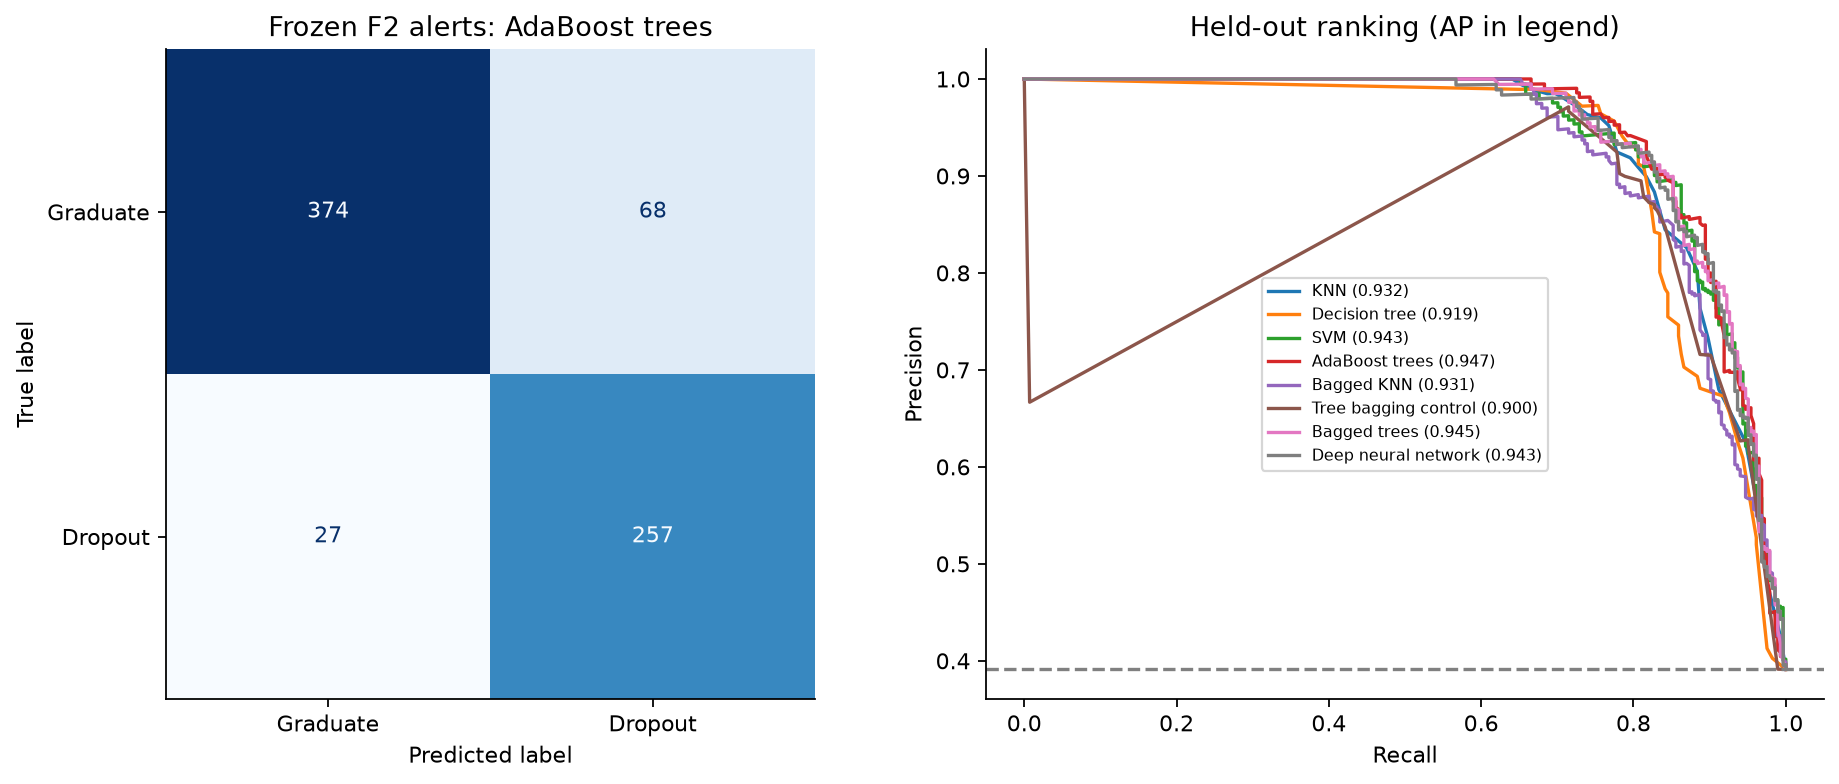
\includegraphics[width=\linewidth]{Images/04_test_classification.png}
    \caption{Held-out confusion matrix at the selected model's fixed F2 threshold
    and precision--recall curves for the evaluated model families.}
    \label{fig:test-classification}
\end{figure}

\subsection{Practical interpretation, uncertainty and limitations}
\emph{Writing prompt: translate the contact budget into students contacted,
recorded dropout cases reached and cases missed. Summarize capacity sensitivity,
conditional bootstrap intervals and calibration (Brier score/log-loss), referring
to optional supporting plots only when needed. Subgroup diagnostics do not
establish fairness; unresolved students have no verified final labels.}

\emph{Writing prompt: answer the question in Section~\ref{sec:problem-statement}.
Build on its scope limitations, adding random rather than temporal evaluation,
development reuse, limited grids and one-course transfer. Explain the need for
prospective and intervention validation without repeating earlier methods.}

% Evidence: test_metrics.csv, capacity_sensitivity.csv,
% conditional_test_intervals.csv, probability_reliability.csv,
% limited_subgroup_diagnostic.csv and summary.json.
% Keep essential numerical evidence in the main report; write tables inline.
